
\subsection{Implicit Runge-Kutta methods\label{rythmos:sec:Implicit-Runge-Kutta-methods}}

We now consider a class of powerful and popular one-step methods for
solving implicit DAEs, implicit Runge-Kutta (RK) methods. The most
general form of implicit RK methods requires the simultaneous solution
of $s$ sets of coupled nonlinear equations that take the form
\begin{equation}
r_{i}(z)=f\left(\dot{X}_{i},\; x_{n-1}+\Delta t\,\sum_{j=1}^{s}a_{ij}\,\dot{X}_{j},\; t_{n-1}+c_{i}\Delta t\right)=0\label{rythmos:eqn:irk_dae_ne}
\end{equation}
for $i=1,\ldots,s$ where $\dot{X}_{i}$ are essentially approximations
to the derivatives $\dot{x}(t_{n-1}+c_{i}\Delta t)$ called \emph{stage
derivatives} and $z=[\dot{X}_{1},\dot{X}_{2},\ldots,\dot{X}_{s}]^{T}$
are the unknowns in this set of equations. After this set of coupled
equations is solved, the state solution $x_{n}$ is given as the linear
combination
\[
x_{n}=x_{n-1}+\Delta t\,\sum_{i=1}^{s}b_{i}\,\dot{X}_{i}
\]
It is clear how to form the residual for the fully coupled system
for $r(z)$ in Eq.~(\ref{rythmos:eqn:irk_dae_ne}) just from individual
evaluations. How the Newton system for such a system is solved will
vary greatly based on the structure and properties of the Butcher
matrix, $a_{ij}$. 

Fully implicit RK methods present somewhat of a problem for developing
general software since they involve the need to solve a fully coupled
system of $s$ sets of equations of the form of Eq.~(\ref{rythmos:eqn:irk_dae_ne}).
Each block $\jac{r_{i}}{z_{j}}=\jac{r_{i}}{\dot{X}_{j}}$ of the full
Jacobian $\jac{r}{z}$ is represented as 
\begin{eqnarray}
W_{ij} & = & \alpha\Jac{f}{\dot{x}}+\beta\Jac{f}{x}\nonumber \\
 & = & \Jac{r_{i}}{z_{j}}=\Jac{r_{i}}{\dot{X}_{j}}\nonumber \\
 & = & \frac{\partial\dot{x}}{\partial\dot{X}_{j}}\Jac{f}{\dot{x}}+\frac{\partial x}{\partial\dot{X}_{j}}\Jac{f}{x}\nonumber \\
 & = & \delta_{ij}\Jac{f}{\dot{x}}+\Delta t\, a_{ij}\Jac{f}{x}\label{rythmos:eq:dridzj_IRK}
\end{eqnarray}
for $i=1,\ldots,s$ and $j=1,\ldots,s$ which is evaluated at the
points $(\dot{x},x,t)=(\dot{X}_{i},\;$ $x_{n-1}+\Delta t\,\sum_{j=1}^{s}a_{ij}\,\dot{X}_{j},\;$
$t_{n-1}+c_{i}\Delta t)$. Note that the iteration matrix, $W$, has
$\alpha=\delta_{ij}$ and $\beta=\Delta t\, a_{ij}$.

When considering a iterative method for solving systems with the block
operator matrix $\jac{r}{z}$, it is easy to see how to use the iteration
matrix $W$ in Eq.~(\ref{rythmos:eq:W}) to implement a matrix-vector
product, but it is not obvious how to precondition such a system.
Clearly a block diagonal preconditioner could be used but the effectiveness
of such a preconditioning strategy is open to question. Other preconditioning
strategies are also possible just given the basic block operators
and this is an open area of research. In some cases, however, it may
be possible to form a full matrix object for $\jac{r}{z}$ but this
is not something that can be expected for most applications.


\paragraph{Semi-explicit IRK methods}

Semi-explicit IRK methods are those IRK methods where the Butcher
matrix, $A$, is lower diagonal and therefore gives rise to a block
lower triangular Jacobian matrix $\jac{r}{z}$. For these types of
methods, the nonlinear equations in Eq.~(\ref{rythmos:eq:dridzj_IRK})
can be solved one at a time for $i=1,\ldots,s$ which is easily accommodated
using a Newton-type method where the Newton Jacobian for each $i$
is given by Eq.~(\ref{rythmos:eq:dridzj_IRK}), which is of our basic
general form, Eq.~(\ref{rythmos:eq:W}).


\paragraph{Singly-Diagonal-implicit IRK methods}

The next specialized class of IRK methods that we consider are singly-diagonal-implicit
IRK methods where the Butcher coefficients in $a_{ij}$ and $c$ give
rise to a lower triangular Jacobian $\jac{r}{z}$ (and hence are also
semi-explicit IRK methods) that has the same nonsingular matrix block
of the form in Eq.~(\ref{rythmos:eq:dridzj_IRK}) along the diagonal.
This, of course, requires that $a_{11}=a_{22}=\cdots=a_{ss}$ and
$c_{1}=c_{2}=\cdots=c_{s}$. (I am not sure that this is possible,
since $c_{i}=\sum_{j=1}^{s}a_{ij}$. The only method that satisfies
this is IRK Backward Euler!? CCO) In this class of IRK methods, significant
savings may be achieved since a single set of linear solver objects
(\emph{i.e.}, operators and preconditioners) can be utilized for the
solution of the fully coupled system. In fact, it may even be possible
to utilize multi-vector applications of the operator and preconditioner
for matrices of the form Eq.~(\ref{rythmos:eq:W}) which can be supported
by many applications. 


\subsubsection{Implicit RK Backward Euler}

\begin{figure}[H]
\centering{}%
\begin{tabular}{cc}
a) $\begin{array}{c|c}
1 & 1\\
\hline  & 1
\end{array}$ & b)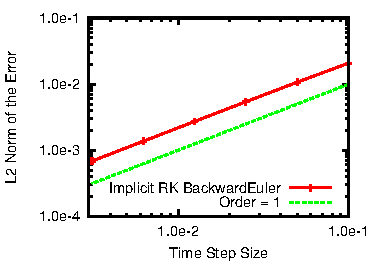
\includegraphics[scale=1.5]{figures/IRK_BackwardEuler}\tabularnewline
\end{tabular}\caption{a) Butcher Tableau and b) Order of accuracy for the SinCos Problem
(Section~\ref{rythmos:sec:SinCos-Problem}) for Implicit RK Backward
Euler.}
\end{figure}



\subsubsection{IRK 1 Stage Theta}

This is a generalization of the midpoint method ($\theta=1/2$).

\begin{figure}[H]
\centering{}%
\begin{tabular}{cc}
a) $\begin{array}{c|c}
\theta & \theta\\
\hline  & 1
\end{array}$ & b)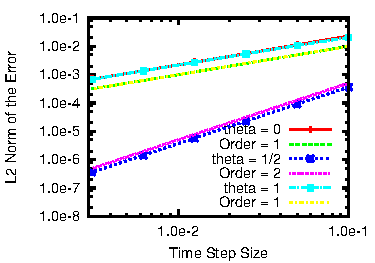
\includegraphics[scale=1.5]{figures/IRK1StageTheta1}\tabularnewline
\end{tabular}\caption{a) Butcher Tableau and b) Order of accuracy for the SinCos Problem
(Section~\ref{rythmos:sec:SinCos-Problem}) for IRK 1 Stage Theta
method.}
\end{figure}



\subsubsection{IRK 2 Stage Theta}

This is a generalization of the trapezoid method ($\theta=1/2$).

\begin{figure}[H]
\centering{}%
\begin{tabular}{cc}
a) $\begin{array}{c|cc}
0 & 0\\
1 & 1-\theta & \theta\\
\hline  & 1-\theta & \theta
\end{array}$ & b)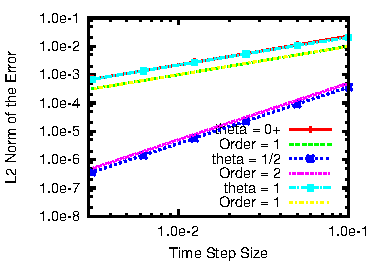
\includegraphics[scale=1.5]{figures/IRK2StageTheta1}\tabularnewline
\end{tabular}\caption{a) Butcher Tableau and b) Order of accuracy for the SinCos Problem
(Section~\ref{rythmos:sec:SinCos-Problem}) for IRK 2 Stage Theta
method.}
\end{figure}



\subsubsection{SDIRK 2 Stage 2 Order}

For $\gamma=(2\pm\sqrt{2})/2$, this method is 2nd order accurate
and L-stable. Other values of $\gamma$ will still produce an L-stable
scheme, but with only be 1st order accurate.

\begin{figure}[H]
\centering{}%
\begin{tabular}{cc}
a) $\begin{array}{c|cc}
\gamma & \gamma\\
1 & 1-\gamma & \gamma\\
\hline  & 1-\gamma & \gamma
\end{array}$ & b)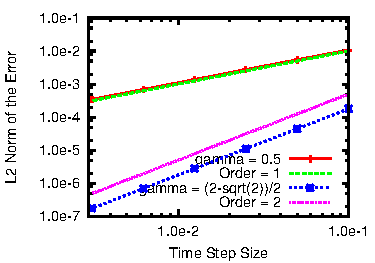
\includegraphics[scale=1.5]{figures/SDIRK_2Stage2Order}\tabularnewline
\end{tabular}\caption{a) Butcher Tableau and b) Order of accuracy for the SinCos Problem
(Section~\ref{rythmos:sec:SinCos-Problem}) for SDIRK 2 Stage 2 Order.}
\end{figure}



\subsubsection{SDIRK 2 Stage 3 Order}

For $\gamma=(3\pm\sqrt{3})/6$, this method is 3rd order accurate
and A-stable. For $\gamma=(2\pm\sqrt{2})/2$, this method is only
2nd order accurate, but is then L-stable.

\begin{figure}[H]
\centering{}%
\begin{tabular}{cc}
a) $\begin{array}{c|cc}
\gamma & \gamma\\
1-\gamma & 1-2\gamma & \gamma\\
\hline  & 1/2 & 1/2
\end{array}$ & b)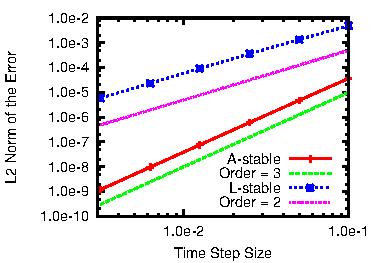
\includegraphics[scale=1.5]{figures/SDIRK_2Stage3OrderLStable}\tabularnewline
\end{tabular}\caption{a) Butcher Tableau and b) Order of accuracy for the SinCos Problem
(Section~\ref{rythmos:sec:SinCos-Problem}) for SDIRK 2 Stage 3 Order.}
\end{figure}



\subsubsection{SDIRK 3 Stage 4 Order}

The coefficients are $\gamma=1/\sqrt{3}\,\cos(\pi/18)+1/2$ and $\delta=(2\gamma-1)^{-2}/6$.

\begin{figure}[H]
\centering{}%
\begin{tabular}{cc}
a)$\begin{array}{c|ccc}
\gamma & \gamma\\
1/2 & 1/2-\gamma & \gamma\\
1-\gamma & 2\gamma & 1-4\gamma & \gamma\\
\hline  & \delta & 1-2\delta & \delta
\end{array}$ & b)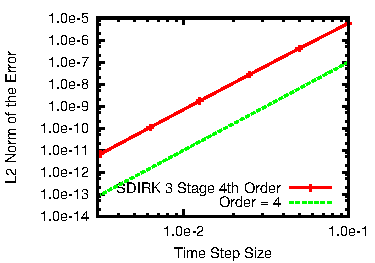
\includegraphics[scale=1.5]{figures/SDIRK_3Stage4Order}\tabularnewline
\end{tabular}\caption{a) Butcher Tableau and b) Order of accuracy for the SinCos Problem
(Section~\ref{rythmos:sec:SinCos-Problem}) for SDIRK 3 Stage 4 Order.}
\end{figure}



\subsubsection{SDIRK 5 Stage 4 Order}

\begin{figure}[H]
\centering{}$\begin{array}{c|ccccc}
1/4 & 1/4\\
3/4 & 1/2 & 1/4\\
11/20 & 17/50 & -1/25 & 1/4\\
1/2 & 371/1360 & -137/2720 & 15/544 & 1/4\\
1 & 25/24 & -49/48 & 125/16 & -85/12 & 1/4\\
\hline  & 25/24 & -49/48 & 125/16 & -85/12 & 1/4\\
 & 59/48 & -17/96 & 225/32 & -85/12 & 0
\end{array}$\caption{Butcher Tableau for SDIRK 5 Stage 4 Order.}
\end{figure}
\begin{figure}[H]
\centering{}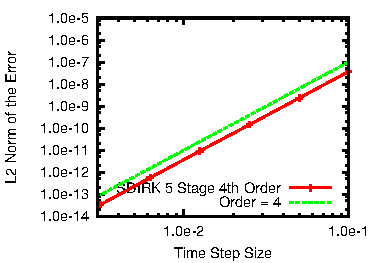
\includegraphics[scale=1.5]{figures/SDIRK_5Stage4Order}\caption{Order of accuracy for the SinCos Problem (Section~\ref{rythmos:sec:SinCos-Problem})
using SDIRK 5 Stage 4 Order.}
\end{figure}



\subsubsection{SDIRK 5 Stage 5 Order}

\begin{figure}[H]
\centering{}$\begin{array}{c|ccccc}
\frac{6-\sqrt{6}}{10} & \frac{6-\sqrt{6}}{10}\\
\frac{6+\sqrt{6}}{35} & \frac{-6+5\sqrt{6}}{14} & \frac{6-\sqrt{6}}{10}\\
1 & \frac{888+607\sqrt{6}}{2850} & \frac{126-161\sqrt{6}}{1425} & \frac{6-\sqrt{6}}{10}\\
\frac{4-\sqrt{6}}{10} & \frac{3153-3082\sqrt{6}}{14250} & \frac{3213+1148\sqrt{6}}{28500} & \frac{-267+88\sqrt{6}}{500} & \frac{6-\sqrt{6}}{10}\\
\frac{4+\sqrt{6}}{10} & \frac{-32583+14638\sqrt{6}}{71250} & \frac{-17199+364\sqrt{6}}{142500} & \frac{1329-544\sqrt{6}}{2500} & \frac{-96+131\sqrt{6}}{625} & \frac{6-\sqrt{6}}{10}\\
\hline  & 0 & 0 & 1/9 & \frac{16-\sqrt{6}}{36} & \frac{16+\sqrt{6}}{36}
\end{array}$\caption{Butcher Tableau for SDIRK 5 Stage 5 Order.}
\end{figure}
\begin{figure}[H]
\centering{}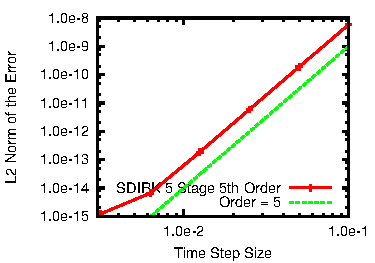
\includegraphics[scale=1.5]{figures/SDIRK_5Stage5Order}\caption{Order of accuracy for the SinCos Problem (Section~\ref{rythmos:sec:SinCos-Problem})
for SDIRK 5 Stage 5 Order.}
\end{figure}



\subsubsection{DIRK 2 Stage 3 Order}

\begin{figure}[H]
\centering{}%
\begin{tabular}{cc}
a)$\begin{array}{c|cc}
0 & 0\\
2/3 & 1/3 & 1/3\\
\hline  & 1/4 & 3/4
\end{array}$ & b)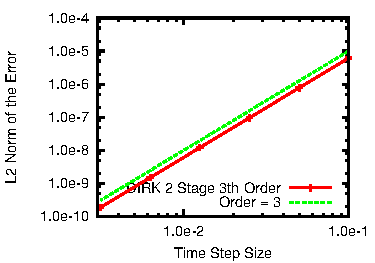
\includegraphics[scale=1.5]{figures/DIRK_2Stage3Order}\tabularnewline
\end{tabular}\caption{a) Butcher Tableau and b) Order of accuracy for the SinCos Problem
(Section~\ref{rythmos:sec:SinCos-Problem}) for DIRK 2 Stage 3 Order.}
\end{figure}

